\documentclass[main.tex,fontsize=8pt,paper=a4,paper=portrait,DIV=calc,]{scrartcl}
% Document
\usepackage[T1]{fontenc}
\usepackage[utf8]{inputenc}
\usepackage[dvipsnames]{xcolor}
\usepackage[nswissgerman,english]{babel} 
\usepackage{hyperref}
\renewcommand{\familydefault}{\sfdefault}

% Format
\usepackage[top=5mm,bottom=1mm,left=5mm,right=5mm]{geometry}
%\setlength{\headheight}{\baselineskip}
%\setlength{\headsep}{0mm}

%\usepackage{scrlayer-scrpage}
%\clearpairofpagestyles
%\chead{{\bfseries\TITLE, \AUTHOR, \pagename~\thepage}}

%\addtokomafont{pagehead}{\upshape}

\usepackage{multicol}
\setlength{\columnsep}{2mm}
\setlength{\columnseprule}{0.1pt}

% Math
\usepackage{amsmath}
\usepackage{amssymb}
\usepackage{amsfonts}

% Code
\usepackage{fancyvrb, etoolbox, listings, xcolor}
%\usemintedstyle{bw}

%\newminted[shell]{bash}{
%fontsize=\footnotesize,
%fontfamily=tt,
%breaklines=true,
%frame=single,
%framerule=0.1pt,
%framesep=2mm,
%tabsize=2
%}
%\newminted{css}{
%breaklines=true,
%tabsize=4,
%autogobble=true,
%escapeinside=||,
%stripall=true,
%stripnl=true,
%}

    \definecolor{lightgray}{rgb}{0.95, 0.95, 0.95}
    \definecolor{darkgray}{rgb}{0.4, 0.4, 0.4}
    \definecolor{purple}{rgb}{0.65, 0.12, 0.82}
    \definecolor{ocherCode}{rgb}{1, 0.5, 0} % #FF7F00 -> rgb(239, 169, 0)
    \definecolor{blueCode}{rgb}{0, 0, 0.93} % #0000EE -> rgb(0, 0, 238)
    \definecolor{greenCode}{rgb}{0, 0.6, 0} % #009900 -> rgb(0, 153, 0)
    \definecolor{teal}{rgb}{0.0, 0.5, 0.5}

\lstdefinestyle{code}{
    identifierstyle=\color{black},
    keywordstyle=\color{blue}\bfseries\small,
    ndkeywordstyle=\color{greenCode}\bfseries\small,
    stringstyle=\color{ocherCode}\ttfamily\small,
    commentstyle=\color{teal}\ttfamily\textit\small,
    basicstyle=\ttfamily\small,
    breakatwhitespace=false,         
    breaklines=true,                 
    captionpos=b,                    
    keepspaces=true,                 
    showspaces=false,                
    showstringspaces=false,
    showtabs=false,                  
    tabsize=2,
    belowskip=-5pt
}



% Images
\usepackage{graphicx}
\newcommand{\pic}{\includegraphics[scale=0.3]}
\graphicspath{{Screenshots/}{../Screenshots}}
\makeatletter
\def\pictext#1#2{%
    \@ifnextchar[{%
    \pictext@iiiii{#1}{#2}%
    }{%
      \pictext@iiiii{#1}{#2}[0.5,0.4,0.3]% Default is 5
    }%
}
\def\pictext@iiiii#1#2[#3,#4,#5]{\begin{minipage}{#3\textwidth}\includegraphics[scale=#4]{#1}\end{minipage}\begin{minipage}{#5\textwidth}#2\end{minipage}}
\def\minipg#1#2{%
    \@ifnextchar[{%
    \minipg@iiii{#1}{#2}%
    }{%
      \minipg@iiii{#1}{#2}[0.3,0.6]% Default is 5
    }%
}
\def\minipg@iiii#1#2[#3,#4]{\vspace{0.8mm}\begin{minipage}{#3\textwidth}#1\end{minipage}\begin{minipage}{#4\textwidth}#2\end{minipage}{\vspace{0.8mm}}}
\makeatother

%\newenvironment{minty}[2]% environment name
%{% begin code
%  \begin{minipage}{#1}
%  \begin{minted}{#2}
%}%
%{% end code
%  \end{minted}
%  \end{minipage}
%  \end{minty}\ignorespacesafterend
%} 

% Smaller Lists
\usepackage{enumitem}
\setlist[itemize,enumerate]{leftmargin=3mm, labelindent=0mm, labelwidth=1mm, labelsep=1mm, nosep}
\setlist[description]{leftmargin=0mm, nosep}
\setlength{\parindent}{0cm}

% Smaller Titles
\usepackage[explicit]{titlesec}

%% Color Boxes
\newcommand{\sectioncolor}[1]{\colorbox{black!60}{\parbox{0.989\linewidth}{\color{white}#1}}}
\newcommand{\subsectioncolor}[1]{\colorbox{black!50}{\parbox{0.989\linewidth}{\color{white}#1}}}
\newcommand{\subsubsectioncolor}[1]{\colorbox{black!40}{\parbox{0.989\linewidth}{\color{white}#1}}}
\newcommand{\paragraphcolor}[1]{\colorbox{black!30}{\parbox{0.989\linewidth}{\color{white}#1}}}
\newcommand{\subparagraphcolor}[1]{\colorbox{black!20}{\parbox{0.989\linewidth}{\color{white}#1}}}

%% Title Format
\titleformat{\section}{\vspace{0.5mm}\bfseries}{}{0mm}{\sectioncolor{\thesection~#1}}[{\vspace{0.5mm}}]
\titleformat{\subsection}{\vspace{0.5mm}\bfseries}{}{0mm}{\subsectioncolor{\thesubsection~#1}}[{\vspace{0.5mm}}]
\titleformat{\subsubsection}{\vspace{0.5mm}\bfseries}{}{0mm}{\subsubsectioncolor{\thesubsubsection~#1}}[{\vspace{0.5mm}}]
\titleformat{\paragraph}{\vspace{0.5mm}\bfseries}{}{0mm}{\paragraphcolor{\theparagraph~#1}}[{\vspace{0.5mm}}]
\titleformat{\subparagraph}{\vspace{0.5mm}\bfseries}{}{0mm}{\subparagraphcolor{\thesubparagraph~#1}}[{\vspace{0.5mm}}]

%% Title Spacing
\titlespacing{\section}{0mm}{0mm}{0mm}
\titlespacing{\subsection}{0mm}{0mm}{0mm}
\titlespacing{\subsubsection}{0mm}{0mm}{0mm}
\titlespacing{\paragraph}{0mm}{0mm}{0mm}
\titlespacing{\subparagraph}{0mm}{0mm}{0mm}

%% format cells
\usepackage[document]{ragged2e}
\usepackage{array, makecell}
\renewcommand{\arraystretch}{2}
\newcommand{\mc}{\makecell[{{m{1\linewidth}}}]}



\begin{document}
\tableofcontents

\lstset{
    language=Java,
    style=code,
}

\newcommand{\TITLE}{Parallel Programming}
\newcommand{\AUTHOR}{Fabio Lenherr}
\setcounter{tocdepth}{1}

\section{Motivation}

\subsection{Moore's Law}
Until now the idea was that more transistors, more GHz, etc means that we can go faster and faster.
However, the issue is that the increases are getting slower and slower, while the workloads are getting increasingly complex with clear need for \emph{multithreading}.

\subsection{Hyperthreading vs Multiple Cores}
\minipg{
Hyperthreading creates the illusion of multiple cores via switching the context of the registers efficiently.\newline
In other words, it just properly streamlines computation similar to JS await/async.\newline
\textcolor{purple}{Note the different instruction set and the same compute core with hyperthreading!}
}{
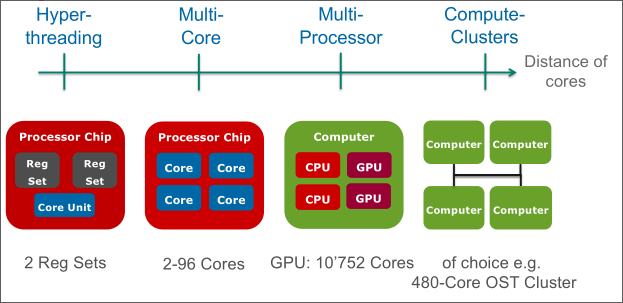
\includegraphics[scale=0.4]{2023_02_20_08_47_23.png}\newline
}[0.55,0.5]

\subsection{Concurrent vs Parallel}
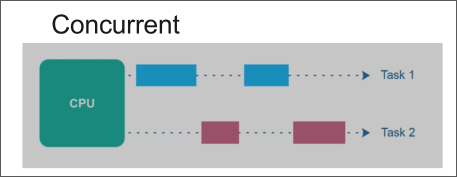
\includegraphics[scale=0.4]{2023_02_20_08_45_03.png}
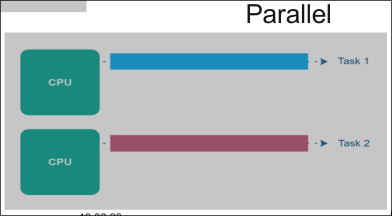
\includegraphics[scale=0.4]{2023_02_20_08_45_08.png}

\subsubsection{Concurrency}
Concurrency has the goal of \emph{simpler programs}, it does this by offering \emph{simultaneous or interleaved(time shared)} execution that accesses shared resources. 

\subsubsection{Parallelism}
Parallelism has the goal of \emph{faster programs}, it does this by decomposition of a program into \emph{several sub-programs}, which can run in parallel on multiple processors or cores.

\section{Parallel Programming in OS Space}

\subsection{Processes and threads}
\minipg{
A process is the instance of a program, while a thread is a subpart of a program, which will then have different callstacks. Meaning that each thread will have it's own callstack but share the same heap!
}{
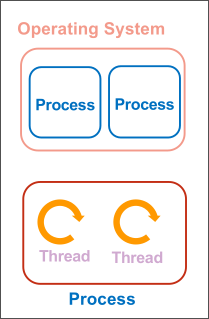
\includegraphics[scale=0.4]{2023_02_20_09_03_15.png}
}[0.7,0.3]\newline
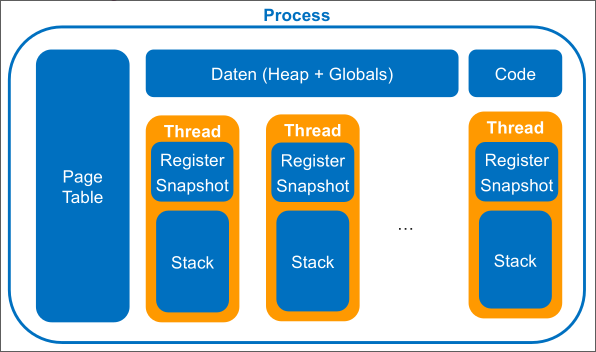
\includegraphics[scale=0.4]{2023_02_20_09_04_01.png}

\subsection{Pros and Cons}
\minipg{
  Cons:
\begin{itemize}
\item \textcolor{red}{Interprocess Communication}
\item \textcolor{red}{Process Management via system calls}
\item \textcolor{red}{Memory isolation}
\end{itemize} 
}{
  Pros:
  \begin{itemize}
  \item \textcolor{green}{Process isolation}
  \item \textcolor{green}{Responsiveness}
  \end{itemize} 
}[0.4,0.4]

\subsection{User threads vs Kernel threads}
\minipg{
  User level threads is a so-called \emph{green thread}, it can't offer true parallelism and is only scheduled by a runtime library or a virtual machine.
}{
  Kernel level thread is the true form of multithreading. \emph{native threads}\newline
It offers context switching via \emph{SW interrupt}.
}[0.25,0.25]

\subsection{Context Switch}
\begin{itemize}
\item \textcolor{purple}{Synchronous}
  \begin{itemize}
  \item \textcolor{black}{Thread waiting for condition}
  \item \textcolor{black}{queues itself as waiting and gives processor free}
  \item \textcolor{black}{locks processor during usage}
  \end{itemize} 
\item \textcolor{purple}{Asynchronous}
  \begin{itemize}
  \item \textcolor{black}{after some defined time the thread should release the processor}
  \item \textcolor{black}{prevent a thread from permanently occupying the processor (solves locks)}
  \end{itemize} 
\end{itemize} 

\subsection{Multi-Tasking}
\begin{itemize}
\item \textcolor{purple}{Cooperative}
  \begin{itemize}
  \item \textcolor{black}{threads must explicitly initiate context switches synchronously at the scheduler at intervals}
  \item \textcolor{black}{scheduler cannot interrupt running thread}
  \end{itemize} 
\item \textcolor{purple}{Preemptive}
  \begin{itemize}
  \item \textcolor{black}{scheduler can interrupt the running thread asynchronously via timer interrupt}
  \item \textcolor{black}{Time-Sliced scheduling: each thread has the processor for maximum time interval}
  \end{itemize} 
\end{itemize} 
\textcolor{red}{Preemptive is used for the most part!!}

\subsection{Thread States}
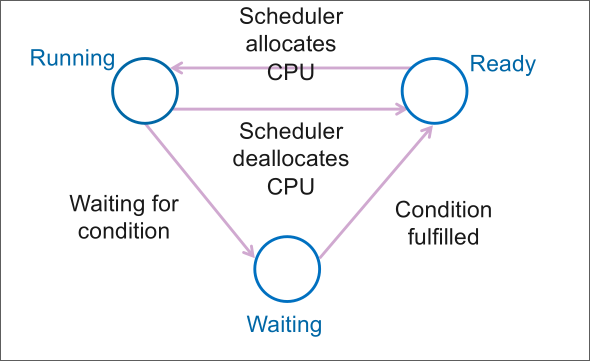
\includegraphics[scale=0.4]{2023_02_20_09_14_43.png}

\subsection{Non-determinism}
When using multi-threading, you can't be sure which thread will be used to complete a task first, meaning that if you print 2 different statements in 2 threads, then you can't be sure of the order in which these statements will be printed.

\section{Parallel Programming in Jafuck}
\subsection{Thread Implementation}
Java implements its own threads which are then linked to the kernel threads.\newline
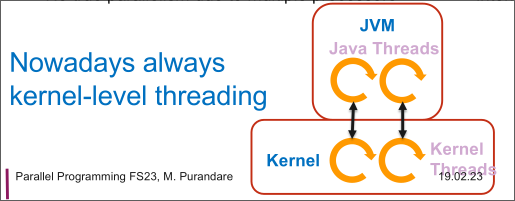
\includegraphics[scale=0.4]{2023_02_20_09_07_53.png}

\subsection{JVM Thread Model}
Java is a single process system -> JVM as one process on the operating system. \newline
\textcolor{purple}{JVM creates a thread at startup which calls main().}\newline
You are then free to call/create more threads as the programmer.

\subsection{JVM Termination}
\begin{itemize}
\item \textcolor{purple}{The JVM runs as long as threads are running, the main function doesn't matter in this case}\newline
  The only exception are so called \emph{daemon threads}, these are threads like the garbage collector, which ofc needs to be ignored for the jvm to EVER end.
\item \textcolor{purple}{You can exit manually via System.exit() or Runtime.exit()}\newline
  Note that this means uncontrolled termination of all threads.
  This can lead to \emph{undefined behavior}.
\end{itemize} 

\subsection{Thread in Java}
A thread in java takes a so called "runnable target", this is an interface that simply defines the type of behavior that can be run inside of a thread. \newline
For example the thread might run something like a lambda.
\begin{lstlisting}
public class Thread implements Runnable {
  private Runnable target;
  public synchronized void start() {
    if (threadStatus != 0)
      throw new IllegalThreadStateException();
    group.add(this);
    boolean started = false;
  }
  public void run() {
    if (target != null) {
      target.run(); 
    }
  }
  public Thread() {
    this(null, null, "Thread-" + nextThreadNum(), 0);
  }
  public Thread(Runnable target) {
    this(null, target, "Thread-" + nextThreadNum(), 0);
  }
}
\end{lstlisting}
\vspace{2mm}
\textcolor{purple}{Note that should a thread cause an exception, the other threads will continue to run!}

\subsection{Example for multithreading in java}
\begin{lstlisting}
public class MultiThreadTest {
  public static void main(String[] args) {
    var a = new Thread(() -> multiPrint("A"));
    var b = new Thread(() -> multiPrint("B"));
    a.start();
    b.start();
    System.out.println("main finished");
  }
  static void multiPrint(String label) {
    for (int i = 0; i < 10; i++) {
      System.out.println(label + ": " + i);
    }
  }
}
\end{lstlisting}
\vspace{2mm}
\textcolor{purple}{Lambdas as well as method references implement the runnable interface}

\subsection{Explicit/Sub-class Thread behavior}
You can explicitly set the behavior of a thread via overriding the run method of the runnable interface.\newline
Note that this means you will implement your own thread!\newline
\begin{lstlisting}
class SimpleLogic implements Runnable {
  @Override
  public void run() {
    // thread behavior
  }
}
var myThread = new Thread(new SimpleLogic());
myThread.start();
\end{lstlisting}
\vspace{2mm}
If you simply with to extend it you can extend the thread class instead:\newline
\begin{lstlisting}
class SimpleThread extends Thread {
  @Override
  public void run() {
    // thread behavior
  }
}
var myThread = new SimpleThread();
myThread.start();
\end{lstlisting}
\vspace{2mm}

\subsection{Thread join}
\minipg{
  This is used when you specifically want another thread to be blocked while another one is running, because you might have a usecase where that one thread needs to fulfill their job.
}{
  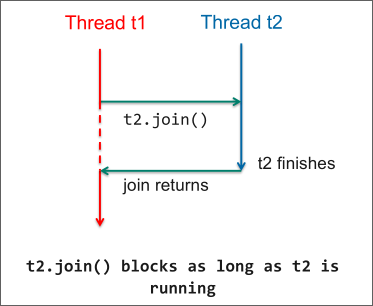
\includegraphics[scale=0.4]{2023_02_20_09_38_24.png}
}[0.6,0.4]
\begin{lstlisting}
var a = new Thread(() -> multiPrint("A"));
var b = new Thread(() -> multiPrint("B"));
System.out.println("Threads start");
a.start();
b.start();
a.join();
b.join();
System.out.println("Threads joined");
\end{lstlisting}
\vspace{2mm}

\subsection{Methods of a thread}
\begin{itemize}
\item \textcolor{purple}{thread.sleep(milliseconds)}\newline
  waits until time has elapsed before becoming ready again -> wait until it is scheduled again to run
\item \textcolor{purple}{thread.yield()}\newline
  thread releases processor and will be ready to be used again -> wait until it is scheduled again to run\newline
  \textcolor{purple}{For newer systems where preemptive multi-tasking is used, there is no need for yield, as allocation if time based either way!}
\item \textcolor{purple}{thread.interrupt()}\newline
  Used for cooperative canceling.\newline
  This is an indication to the thread that it should stop current operation and do something else.\newline
  This can be used by the programmer to decide how the thread will respond to an interrupt, however it is common for the thread to terminate on interrupt.
\end{itemize} 

\section{Thread Synchronization}
This is the try to get a synchronized order of running threads.\newline
In other words, we sacrifice some performance for the sake of deterministic running of threads.

\subsection{Race Condition}
\minipg{
When 2 threads try to access, more specifically \emph{write} to the same variable at the same time, you might lose one of these writes if their write overlaps.\newline
This is yet another reason to just use rust, as this is handled via the borrow rules!\newline
\emph{Only 1 mutable reference at a time, OR, unlimited immutable references.}
}{ 
  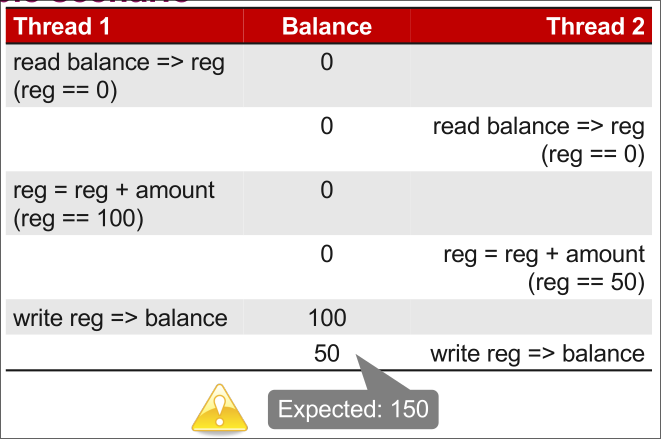
\includegraphics[scale=0.3]{2023_02_27_08_31_29.png}
}[0.6,0.4]

\subsection{Critical Section}
This is a certain part of a job that must be done in sequence, for example a \emph{transaction of a bank}.\newline
\textcolor{purple}{The solution might seem easy, why not just create a locked variable, however, if you do this then you will run into the same problem, When exactly will the lock be written? The same race condition can apply here.} 

\subsection{Synchronized methods in java}
\textcolor{purple}{In java you can mark a method as synchronied to make sure that you will not run into race conditions.}
\begin{lstlisting}
class BankAccount {
  private int balance = 0;
  // function that may not be "truly" multithreaded
  public synchronized void deposit(int amount) {
    this.balance += amount;
  }
}
\end{lstlisting}
\textcolor{purple}{When using these methods, make sure that \emph{ALL} methods that need to be synchronized also have this flag.\newline
In other words if you have a withdraw function and a deposit method, make sure both are marked as synchronized}

\subsubsection{Synchronized Blocks}
You can also just specify a block to be synchronized.\newline
\textcolor{purple}{In this case you need to pass a class to be locked!}
\begin{lstlisting}
class BankAccount {
  private int balance = 0;
  public void deposit(int amount) {
    synchronized(this) {
      // specify the this object to be locked
      this.balance += amount;
    }
    System.out.println("Deposit done");
  }
}
\end{lstlisting}
Similar, you can make locks on both \emph{Classes and Objects}. 
\begin{lstlisting}
class Test {
  synchronized void f() { ... } // object lock
  static synchronized void g() { ... } // class lock
}
class Test {
  void f() { // object lock
    synchronized(this) { ... }
  }
  static void g() { // class lock
    synchronized(Test.class) { ... }
  }
}
\end{lstlisting}

\subsubsection{Multiple locks}
\textcolor{purple}{When a method is recursive and synchronized, the method will have multiple locks, of these, it needs to release all of them at the end for the next thread to aquire the locks.}\newline
In other words, the locks are like refcounting. 
\begin{lstlisting}
synchronized void limitedDeposit(int amount) {
  if (amount + balance <= limit) {
    deposit(amount);
  }
}
synchronized void deposit(int amount) { … }
// will free the locks once all of the calls are done.
\end{lstlisting}

\subsubsection{wait()}
\textcolor{purple}{The wait method will release the lock and regain it after the thread has received a \emph{wake up call}.}
\begin{lstlisting}
class BankAccount {
  private int balance = 0;
  public synchronized void withdraw(int amount) throws InterruptedException {
    while (amount > balance) {
      wait(); // release lock and go into waiting mode
    }
    balance -= amount;
  }
}
public synchronized void deposit(int amount) {
  balance += amount;
  notifyAll(); // wakeup all waiting threads!
}
\end{lstlisting}
\textcolor{purple}{As you can see, if a thread goes into waiting mode and does not receive a wakeup call, it will not start again.\newline
This can cause \emph{deadlocks}, as you might have multiple threads waiting for something to happen, but nothing ever will.}
\begin{itemize}
  \item \textcolor{orange}{notifyAll} wakes up \emph{all} waiting threads \emph{in the inner waiting room}
  \item \textcolor{orange}{notify} wakes up \emph{a random waiting thread} which is in the \emph{inner waiting room}\newline
\end{itemize} 
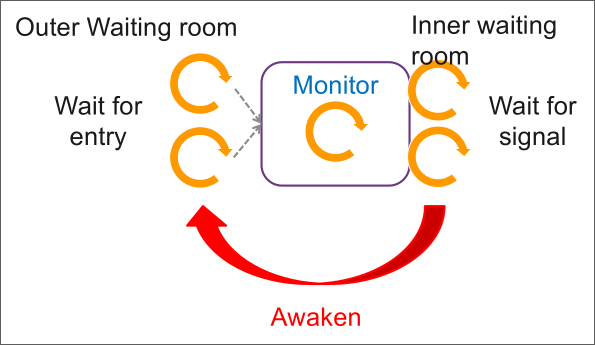
\includegraphics[scale=0.4]{2023_02_27_09_36_15.png}
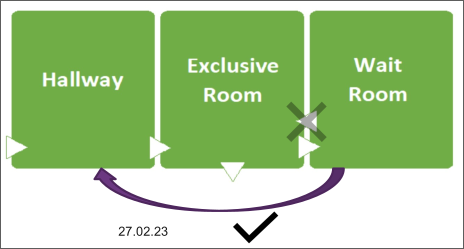
\includegraphics[scale=0.4]{2023_02_27_09_37_23.png}
In other words, wait() will put the thread in the hallway, the operating system will then put the thread into the exclusive room after it is scheduled. From here it can be awoken early with \emph{notifyALL}, or it can wait until it is in the proper waiting room, where it can be called with \emph{notify()}.

\subsubsection{Traps with Monitors}
\textcolor{purple}{Trap 1: IF}
\begin{lstlisting}
public synchronized void put(T x) throws InterruptedException {
  if (queue.size() == capacity) {
    wait(); // await non-full
  } // oops we only waited once, if the capacity is still to small we now have a problem!
  queue.add(x);
  notify(); // signal non-empty
}
// instead!
while (!condition) {
  wait(); // this makes sure that we will wait even after the thread gets another lock!
}
\end{lstlisting}
\textcolor{purple}{Trap 2: Overtaking}\newline
\textcolor{teal}{Here the issue is that if you use notify(), you are going to call a random thread, in case you need serialization, you will not be achieving this with notify(), \emph{instead use notifyALL()!}}
\begin{lstlisting}
// ...
queue.add(x);
notify(); // signal non-empty
\end{lstlisting}
\textcolor{purple}{Trap 3: Eternal Wait}\newline
\textcolor{teal}{Here the issue is that with a single notify(), you might awaken a thread that will then also wait for another condition, which will not notify any other thread, meaning that there is no further notify chaining.\newline
You will now wait for something that will never be done, good job :)}

\subsection{Spurious Wake-up}
\textcolor{purple}{This is a OS specific feature, for example for POSIX operating systems.}\newline
Here the thread can \emph{spuriously awaken without a specific notify}, this is something that you as a developer have to guard against!

\end{document}
